\documentclass[11pt]{article} % For LaTeX2e
\usepackage{times}
\usepackage{url}
\usepackage{natbib}
\usepackage{amsmath}
\usepackage{amsthm}
\usepackage{amssymb}
\usepackage{graphicx}

\addtolength{\textwidth}{2cm}
%\addtolength{\textwidth}{1cm}
\addtolength{\textheight}{2cm}
%\addtolength{\textheight}{1cm}
\addtolength{\topmargin}{-1cm}
\addtolength{\oddsidemargin}{-1cm}
\addtolength{\evensidemargin}{-1cm}

\title{Deep Learning \\ NATURE Review Article}

\author{Target: 4500 words, 4 main figures and less than 100 citations (8 pages total)}

\begin{document}

\maketitle

\begin{abstract}
Deep learning is currently the most exciting area of machine learning
because it has dramatically improved the state-of-the-art in speech
recognition, object recognition and object detection.  It is also being
remarkably successful at many other tasks such as language modeling
(predicting the next word in a sentence) and predicting the activity of
potential drug molecules.  In addition to its impressive successes for
perceptual tasks, deep learning is currently on the verge of beating the
state-of-the-art in Machine Translation and is likely to become the method
of choice for this task over the next few years.
There is widespread interest in deep learning because it is so good at
extracting structure from very large datasets and it appears to be very
widely applicable. For example, it was named as one of the top ten new
technologies of 2013 by MIT Technology Review. This review explains some
of the main underlying concepts and current applications of deep learning,
and closes with perspectives for future research in this area.
\end{abstract}

{\em 
We plan to organize this review chronologically, but with forward looking
 comments. We will start with the excitement over the backpropagation
 learning algorithm for multilayer neural networks in the 1980's and
 explain why these networks did not live up to the very high expectations
 that people had for them.  Given our current knowledge, the real reasons
 for the disappointments of the 1990's are now clear: people radically
 underestimated the amount of data and the amount of computation that were
 required to demonstrate the power of this type of learning algorithm.
}

\section{DISTRIBUTED REPRESENTATIONS AND DEEP LEARNING}

Traditional approaches to pattern recognition required engineers to design
a feature extractor that turns raw sensory data into representations that
are suitable for conventional machine learning algorithms. Deep learning
algorithms aim to replace these hand-crafted representations by learned
ones, taking advantage of the information implicitly available in
data. Deep learning research aims at discovering mechanisms for learning
multiple levels of representation of the data, with higher levels of
representation representing more abstract features that simplify further
processing, e.g., for tasks such as object recognition, speech recognition,
or translation from one language to another.

The kind of representations extracted by deep learning have two central
characteristics: they are distributed representations and they are deep
representations. A distributed representation is composed of features that
are not mutually exclusive, such that the number of configurations of
values of these features grows exponentially with the number of
features. Imagine for example that these features are binary, i.e., each
can take only one of two values. Then up to configurations of these bits
are possible, thus carving up to regions in the input space. Yet the number
of free parameters required to carve this very rich partition of the input
space grows only linearly with , since feature (e.g., a neuron) comes with
its set of parameters (e.g., synaptic weights into the neuron). This is in
contrast with the majority of other machine learning approaches, in which
the number of parameters (and thus of examples) necessary to distinguish
input regions grows linearly with , instead of logarithmically. This
includes most clustering techniques, nearest-neighbor techniques, most
kernel-based non-parametric approaches, and decision trees. These
approaches can be plagued by the curse of
dimensionality~\citep{Bengio-localfailure-NIPS-2006-small,Bengio-decision-trees10}:
in rich domains such as images and text, the number of configurations of
interest of the observed variables is exponentially large, making it very
difficult to generalize. As argued in \citet{Bengio-book-2009,Montufar+Morton-2014,Montufar-et-al-NIPS2014},
distributed representations potentially have a very large
statistical advantage, in the sense that fewer examples might be needed to
achieve the same ability to generalize to new cases, or that markedly
better generalization can be obtained for the same number of training
examples.


Similarly to a deep neural network where the output of one group of neurons
is the input of another group, etc, if the learned function is obtained as
a composition of many non-linearities, then very rich functions can be
represented which can carve out exponentially more regions in input space
than a shallow architecture~\citep{Montufar-et-al-NIPS2014}. In both cases (distributed
representations and depth of representation), the mathematical arguments
rely on the ability to compose many pieces in order to get access to a very
rich class of computations. More abstract features can be computed in terms
of a composition of lower-level ones more efficiently than if these
abstract features had to be spelled out more explicitly, by enumerating all
the cases or templates that correspond to that feature. Whereas previous
theoretical work on neural networks showed that two layers (i.e. a single
hidden layer) was enough to approximate any continuous function, recent
theoretical results show that a shallow architecture may need to be very
fat where a deep one can much more efficiently (with fewer computations)
represent the same function~\citep{Bengio+Delalleau-ALT-2011-small,Montufar-et-al-NIPS2014}.

However, one has to keep in mind that not every function can be efficiently
represented with a distributed representation or with a deep
architecture. In other words, using deep learning corresponds to relying on
a broad a priori belief about the underlying data in order to achieve good
generalization to new cases. The prior is basically that the data we
observe can be explained by the combination of a limited set of factors or
features, and that one can learn about each of these factors or features
without having to see all the configurations of the other
ones. Fortunately, this very broad assumption seems to hold well in AI
tasks involving images, sounds and language.




\section{THE BACK-PROPAGATION ALGORITHM AND ITS APPARENT LIMITATIONS}

{\em 
We will explain the core issue of hand-engineering features versus learning
 features automatically from data and show how backpropagation learns
 features. We will describe the most successful application of the
 80's/90's which was reading hand-written digits. We will also explain
 "distributed representations[a]" and illustrate them by showing how
 backpropagation can be used to convert words to vectors of meaningful
 features which are now very widely used in natural language applications.
  We will show how backpropagation through time can be used to learn
 recurrent neural networks and we will explain the vanishing/exploding
 gradients problem that makes this type of learning difficult.
}

\subsection{How backpropagation works}

Many machine learning algorithms are designed around the minimization of a
training criterion, such as the error made on a set of training
examples. Monitoring the average value of that training criterion over
training examples tells us if learning is progressing, and learning
algorithms involve a method to modify parameters of the model (such as the
synaptic efficacies of an artificial neural network) so as to gradually
improve this training criterion. The most basic approach relies on
computing or estimating the derivatives of the training error with respect
to parameters, which tells us, for each parameter, what would happen to the
error made by the neural network if that parameter was increased
slightly. We call all these derivatives the error gradient and it indicates
in which direction to move the parameters. If the gradient on a particular
synaptic weight is positive, it means that one should decrease the weight
in order to decrease the error made. Instead, if the gradient is negative,
it means that increasing the weight would decrease the error, and so that
is what we should do.


Backpropagation is an algorithm to compute these derivatives, when the
function computed by the neural network is the composition of many
elementary computations, as in the case of a deep multi-layer
architecture. It relies on the idea that if we know in what direction to
change the outputs of artificial neurons at one layer, we can figure out
how to change the synaptic weights into these neurons so as to reduce the
error. Importantly, these error gradients on the neurons outputs at one
layer also tell us how to obtain the error gradients at the previous
layer. This is obtained through application of the chain rule for
derivatives, which specifies how to compute derivatives through a
composition of functions.  Many different types of fixed or learned
modules can thus be composed and trained end-to-end~\citep{LeCun98} 
to form complex systems that perform
tasks such as speech recognition, document analysis, or machine
translation.

\begin{figure}[H]
\centerline{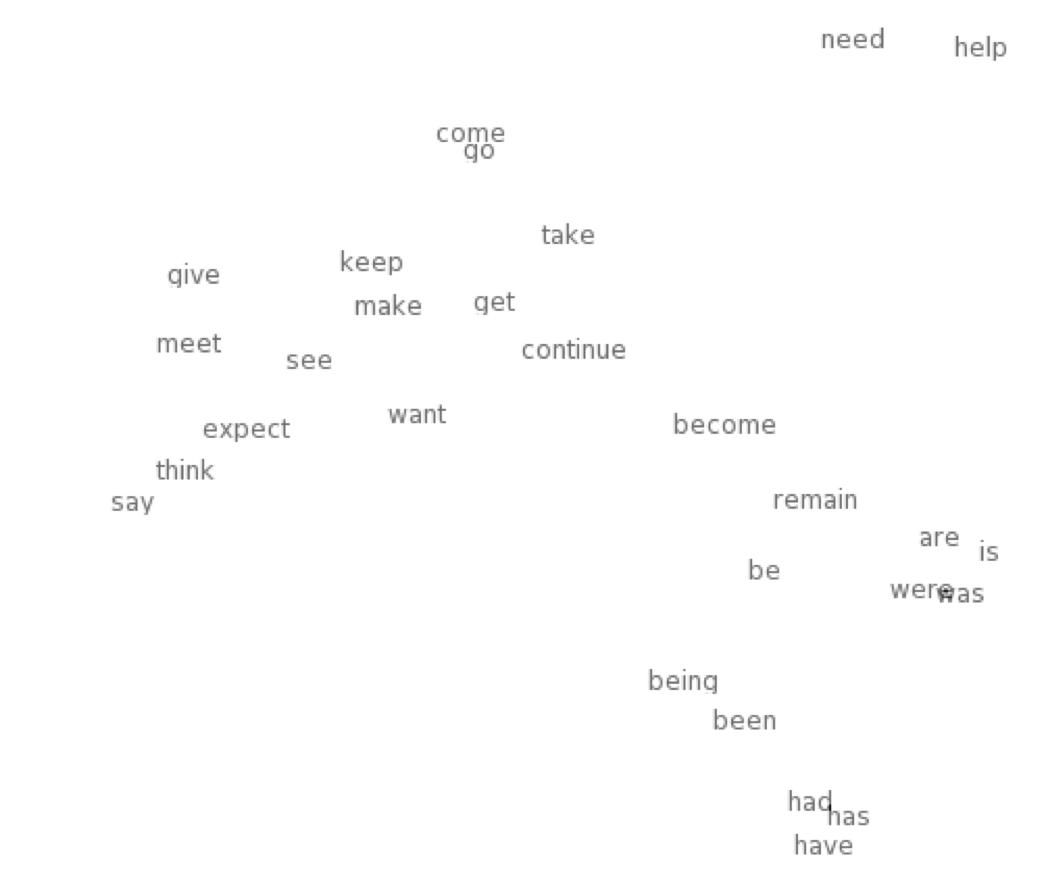
\includegraphics[width=0.7\linewidth]{word-embeddings.png}}
\caption{Illustration of word representations learned for modeling
language, non-linearly projected to 2-D for visualization.}
\end{figure}



\subsection{Neural word representations}

A nice example of the use of backpropagation is how it can be used to learn
representations for symbols, such as words. ~\citet{Hinton86b} introduced the idea
of learning a distributed representation for symbols and \citet{BenDucVin01-short}
showed how to combine the idea of learning a distributed
representation for each word with the task of modeling the probability
distribution of sequences of words (sentences from a corpus of text). We
have basically the composition of two components: (1) mapping each of the
previous words in the sentence to their representation, and (2) mapping the
concatenation of these representations to a prediction for the
representation of the next word, from which one can compute its
probability.  Like in other applications of back-propagation, there seems
to be a chicken-and-egg problem, in the sense that the mapping (2) relies
on the word representations in (1), while it is the objective of achieving
the task performed by (2) that pushes the word representations in (1) to be
meaningful. It works because both are learned together, by a large number
of small gradual changes. The result is that words that are semantically
similar in the sense of being exchangeable end up nearly with the same
representation: one can replace ``funny'' by ``comical'' in many sentences and
the sentence remains plausible, so these two words have almost the same
representation. Similarly, ``Tuesday'' and ``Wednesday'' are exchangeable in
most sentences, so they end up very close to each other, while ``dog'' and
``cat'' are not always exchangeable but often are, so they are not too far
from each in that space. Furthermore, the way in which the representations
for related words differ ends up being also meaningful: the difference
between the representation for ``king'' and the representation for ``queen'' is
very close to the difference between the representation for ``man'' and the
representation for ``woman'' \citep{Mikolov-et-al-ICLR2013}. The system has discovered
features, such as gender in the above example, and learned to map each word
to its proper features.


\iffalse
\begin{figure}[H]
\centerline{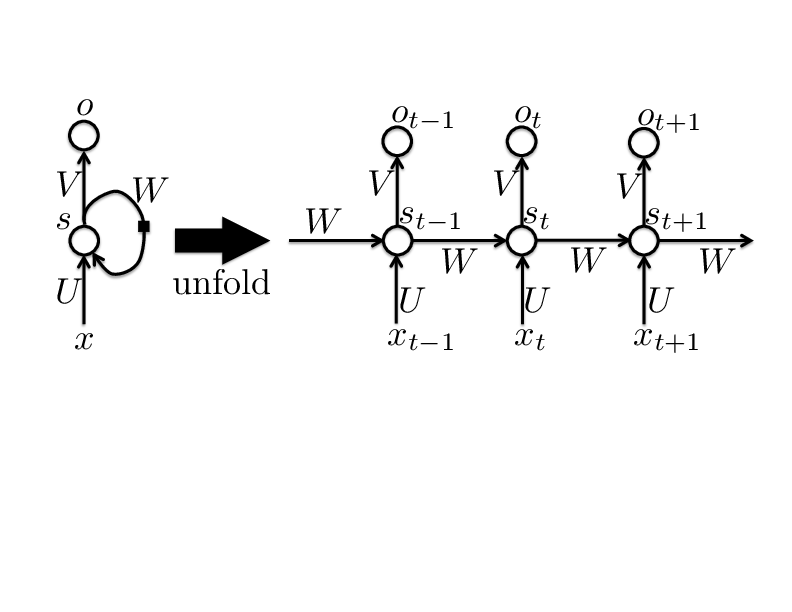
\includegraphics[width=0.7\linewidth]{fig-hidden-recurrence-rnn.png}}
\caption{(a better figure can be made)}
\end{figure}
\fi

\subsection{Training recurrent nets}

A particularly interesting and general form of neural network is the
recurrent neural network. It can process temporally structured data, by
scanning through it just like humans and animals do: at each time step the
neural network “sees” as input the next element of the sequence, and
changes its internal state , which is therefore a representation of all the
previously seen elements . We can think of the brain as an enormous
recurrent neural network: the activity of all the neurons at a given time
constitutes the state of the brain recurrent network. Your next visual
saccade may provide the next input to the brain’s recurrent network. A
recurrent network can also have outputs, corresponding to actions or
predictions, and the training objective for a recurrent network is
obtained from these values. For example, a recurrent network for language
modeling has output units that predict the next word in the sequence. At
each time step it gets a new word as input and updates its state. Such a
network can also “imagine” a plausible sequence, which makes it a so-called
generative model.  At each time step, given the current state, the network
makes a probabilistic guess about the next word, say, given the previous
words. By randomly choosing the next word according to these probabilities,
one more element is added to the sequence, which becomes an input used to
update the state and predict the next word. Begin by thinking of the first
word to type, then type it. In general, given the words already typed,
think of the next word to type that would be compatible with those you
already wrote, etc. Maximizing the training criterion for such a recurrent
network also maximizes the probability that the recurrent network will
generate sequences such as those in the training corpus.


\subsection{The challenge of training very deep nets and recurrent networks over long sequences}


One can view a recurrent network as a very deep neural network if we
consider each time step as one layer (right hand side of Figure xx). Deep
networks and recurrent networks are both very powerful because they can
represent very complex and non-linear functions formed by a long chain of
compositions. However, for the same reason, they are intrinsically
difficult to train, from the point of view of numerical
optimization. Composing many non-linear functions yields an even more
non-linear function. In cases where most of the composed functions had
small derivatives (a small change in input yields a smaller change in
output), the error gradient vanishes because it is the product of the
derivatives computed for each layer or each time step. In other cases (but
more rarely), a very small change in the parameters will yield a large
change in the error, and we have exploding gradients. Both of these
conditions throw off gradient-based optimization, which relies on
back-propagation to compute gradients. Although there has been substantial
progress to train recurrent neural networks (see a review of these
techniques~\citep{Pascanu+al-ICML2013-small}, it remains a challenge to deal with long
sequences where there are so-called long-term dependencies: a small change
in the input at some point in the sequence could have a strong impact on
the correct output much later in the sequence.


\section{DEEP UNSUPERVISED LEARNING}

{\em
We will explain the breakthrough that occurred in 2006 when an effective
 new way of learning multiple layers of features was discovered. The idea
 is to learn the layers one at a time with the objective being to build a good
 model of the correlations between feature activities in the previous layer
 (or the input).  After this layer-by-layer unsupervised "pre-training" to
 discover features, backpropagation works very well for fine-tuning the
 features that have already been discovered.  Will we describe several
 variations of the pre-training methods.
}

\begin{figure}[H]
\centerline{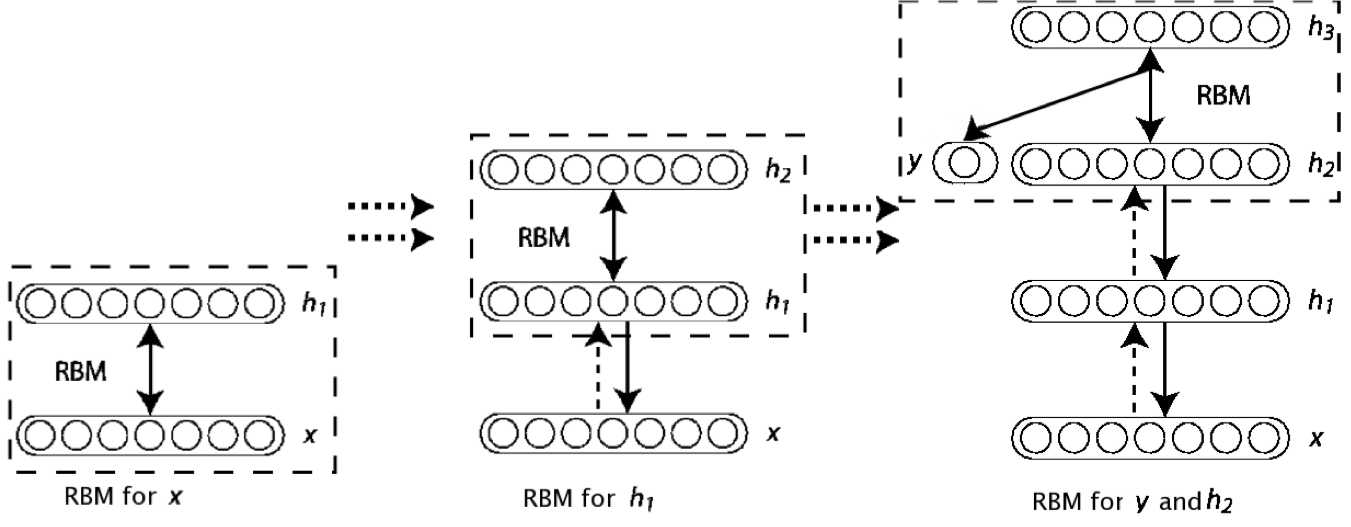
\includegraphics[width=0.7\linewidth]{stacked-rbms.png}}
\caption{stacking RBMs}
\end{figure}

\subsection{Unsupervised pre-training}

Prior to 2006, most attempts at training multi-layered neural networks with
more than a few layers had failed and did not have any impact. However, a
few researchers, including the authors of this paper, continued searching
for ways to train deep neural networks, and many of them joined forces in a
Canadian research program with international nodes, called NCAP (Neural
Computation and Adaptive Perception), funded by the Canadian Institute For
Advanced Research (CIFAR), and headed by Geoff Hinton (and since 2014, by
Yoshua Bengio and Yann LeCun). In 2006, these researchers put out several
papers~\citep{Hinton06, Bengio-nips-2006-small,ranzato-07-small} outlining a general strategy for taking advantage of
unsupervised learning of individual layers of a deep neural network in
order to initialize (or pre-train) a deep supervised network. Unlike
supervised learning, unsupervised learning only needs to look at the input
of the neural network, not the targets that we want to associate with these
inputs, so it can take advantage of large quantities of unlabeled data (for
which no target is given, which have not been examined and tagged by
humans) and even data associated with other tasks (see ‘transfer learning’,
below).  These unsupervised learning algorithms produce a new representation
of the data by learning the synaptic weights of a new layer of neurons that
map the raw input (or the output of the previous layer) to a new set of
learned features. Whereas traditional machine learning is based on
hand-crafted features, deep learning aims at taking advantage of data
(potentially unlabeled) in order to discover good features. This raises a
very good and difficult question: what is a good representation? Different
deep learning algorithms answer this question in different ways, but the
general idea is that a good representation makes it easier to learn further
dependencies, either between the features themselves (e.g., they are
independent or just linearly related to each other), or between the
features and some target variables (if we want to predict some categories,
given these features). An important ingredient of these 2006 papers is
that, although the job of learning a good representation is difficult,
unsupervised learning allows to improve a representation by iteratively
transforming previous representations. In these experiments, a new
Restricted Boltzmann Machine or auto-encoder is trained for creating the
next layer, and the representation learned can be used as input to train
the next layer similarly. After adding several such layers, one can
consider the overall mapping from input to top-level representation as the
initialization for a deep supervised neural network, which is further
trained with respect to the supervised objective (e.g., minimizing
classification error). We call this stage supervised fine-tuning because
all the layers are adjusted with respect to a single global objective,
after having been initialized from layer-wise unsupervised pre-training.

\subsection{Semi-supervised learning and transfer learning}


Most data that would be available to a learner does not come with
human-verified labels providing the desired characterization of its
content. This is true for humans as well as for machines and has motivated
machine learning methods called semi-supervised learning, in which both
labeled data and unlabeled data are exploited. One way in which unlabeled
data can be exploited is by helping to learn good representations, that
capture the underlying factors of variation present in the data. An example
of this approach is the unsupervised pre-training scheme discussed above
(which does not require labels), followed by supervised fine-tuning (on the
labeled examples). An interesting side-effect of learning good
representations (whether in an unsupervised, semi-supervised, or supervised
way) is that they tend to be useful for learning new but related tasks. For
example, in 2011 we participated in two international transfer learning
competitions~\citep{UTLC+LISA-2011-small,Goodfellow+all-NIPS2011} and won thanks to unsupervised learning of
representations. The representations were learned using a large dataset
corresponding to some categories, while they were to be used as input for
training a linear classifier on a very small number of examples of other
categories. Because the different categories shared underlying factors of
variation (for example, many different object categories share
similarly-shaped parts and sub-parts), the models that benefited from the
pre-trained representations performed considerably better than those which
did not, and yielded very good generalization with only a few labeled
examples of the new categories. We believe that such transfer works well
when the learned representations capture high-level abstractions, some of
which may be relevant for both the training tasks and the test tasks. The
same process proved successful in the context of domain adaptation~\citep{Glorot+al-ICML-2011-small},
where the task was the same (sentiment analysis) but the input
distribution was different (the training domain might include comments
about movies and books, while the test domain could include comments about
music or electronic products).


\section{DEEP SPEECH RECOGNITION}


{\bf Geoff}

{\em We will explain the acoustic modeling problem in speech recognition and
 desribe how initial results in 2009 using pre-training on the TIMIT
 dataset led to huge improvement in acoustic modeling over the next few
 years. Acoustic models based on deep neural networks are now used in most
 smart phones.  We will address the issue of when pre-training is needed
 and when it is unneccessary.
}

\section{DEEP CONVOLUTIONAL NETWORKS FOR OBJECT RECOGNITION AND DETECTION}


{\bf Yann}


\section{DEEP RECURRENT NEURAL NETWORKS FOR MACHINE TRANSLATION}


{\bf Yoshua}


Machine translation is an appealing task because it seems that in order to
do it well, one has to capture a lot of the subtleties of meaning. Unlike
object recognition and speech recognition, it goes beyond pure sensory
perception and into the world of symbols where many researchers believed
that neural networks would be unable to rival more conventional AI
approaches.


In 2014, deep learning techniques, in particular those based on recurrent
networks, made rapid
progress~\citep{Devlin-et-al-ACL2014,Bahdanau-et-al-arxiv2014,Sutskever-et-al-arxiv2014}. Systems
based on deep learning have now reached and in some cases passed the
state-of-the-art, e.g., for English-French and English-Arabic. Machine
translation technology had matured into a fairly complex pipeline over the
previous decade, involving many separately trained pieces and much
domain expertise. Only a few parameters were trained to optimize a global
objective, and the core elements of deep learning, i.e., multiple layers of
distributed representations, were lacking. Instead, the core component of
traditional machine translation, as in earlier language modeling systems,
relied on counting co-occurences of short phrases with their presumed
translated phrases. This makes it very difficult for the learned system to
generalize to semantically similar phrases that have not been seen in the
training set. Because the number of ways of saying the same thing grows
exponentially with the size of the vocabulary and the length of the phrase,
this approach suffers from the curse of dimensionality: there are too many
possible configurations of the variables of interest (here, words) to be
able to observe all of the relevant configurations often enough. The
initial goal of deep learning researchers was to use distributed
representations to replace or complement some of the pieces of existing
machine translation systems, but more recent work aims to replace the
entire system with a set of recurrent neural networks that are trained
end-to-end~\citep{Bahdanau-et-al-arxiv2014,Sutskever-et-al-arxiv2014}.
We now give a simplified sketch of how this can be done.

For each language there is a recurrent encoder network that reads the words
in the source phrase or sentence one at a time. Each word is converted to a
distributed representation and the hidden state of the encoder network is
then recomputed from this word representation and the previous hidden
state. The final hidden state of the encoder network then becomes the
initial hidden state of the decoder network for the target language and
this decoder network produces a probability distribution for the first word
in the translation. If we pick from this distribution and feed the chosen
word into the decoder network as input, the decoder network will produce a
probability distribution over possible second words conditioned on the
chosen first word. If we keep repeating this process, the decoder network
defines a probability distribution over complete translations and the
encoder and decoder network can both be trained by backpropagation through
time to maximize the probability assigned to the translation that is given
in the training set. An attention mechanism can be defined to
learn to make the connection between the input and output sequences
and improve performance on long sentences~\citep{Bahdanau-et-al-arxiv2014}.

It turns out that word representations learned by recurrent neural networks
that are trained to translate are better at capturing the semantic
similarity judgements made by humans than other representations of words,
including those derived by learning a neural language model~\citep{Hill-et-al-2014}.

\section{DEEP MINDS}


{\bf Geoff}

\section{FUTURE DIRECTIONS}


Widespread application of the existing DREDNET technology:  Predicting activities of molecules, detecting particles, controlling robot motion ...


Deep Boltzmann machines (just mention undirected models!).


Intelligent fixations for vision. 


Convolutional capsules (just a couple of sentences).\\


{\bf PROVISIONAL LIST OF FIGURES, TABLES AND BOXES}

In addition to the above:\\

One box explaining the backpropagation algorithm for computing error derivatives.\\


One box explaining stochastic gradient descent.


....




{\bf KEY REFERENCES (dotted lines separate refs for each heading above)}\\
(some of the conference papers here are awaiting review as journal papers and those refs will be updated if accepted.)


Rumelhart, Hinton \& Williams backprop paper 
\citep{Rumelhart86b}

Lecun et al Document analysis with CNN.
\citep{LeCun+98}

Robinson RNN for speech
\citep{Robinson+Fallside91}

Neuro probabilistic language models
\citep{BenDucVin01-short}

----------------


Hinton et al  Deep belief net paper.
\citep{Hinton06}

Hinton et. al. Speech recognition with DNNs, Signal Processing Magazine 
\citep{Hinton-et-al-2012}

Graves et al RNNs for speech
\citep{Graves-et-al-ICASSP2013}

----------------


al. et. Lecun  Overfeat paper
\citep{Sermanet14}

Krizhevsky, Sutskever and Hinton, Imagenet paper
\citep{Krizhevsky-2012-small}

al. et. Lecun face recognition paper?
 
----------------


Hochreiter ref?
\citep{Ciresan-2010}

Graves et. al. paper showing that LSTM's work for handwriting recognition.
\citep{Graves-et-al-2009}

------------------
MT papers:

\citep{Devlin-et-al-ACL2014,Bahdanau-et-al-arxiv2014,Sutskever-et-al-arxiv2014}

-----------------


Deep mind NIPS paper on videogame player.
\citep{Deepmind-atari-arxiv2014}


\bibliography{strings,ml,aigaion}
\bibliographystyle{natbib}

\end{document}

